\documentclass{nature}

\usepackage[english]{babel}
\usepackage[utf8]{inputenc}
\usepackage[T1]{fontenc}
\usepackage{amsmath,amssymb}
\usepackage{graphicx}
\usepackage{booktabs}
\usepackage{siunitx}
\usepackage{hyperref}
\usepackage{xcolor}

\begin{document}

\title{Supplementary Information: Rapid Epitope-Targeted Nanobody Design via Differentiable Distogram Optimization with ESMFold2}

\maketitle

\section{Supplementary Tables}

\subsection{Table S1: Parameter sweep results}

Systematic parameter sweep on RBD/VHH72 (6WAQ). All runs use ESMFold2-Fast (721M) on MPS, single seed. ``Bounce'' indicates cdr$\to$epitope oscillation magnitude.

\begin{table}[htbp]
\centering
\caption{Parameter sweep on RBD/VHH72. wt\_logit is the key bottleneck.}
\begin{tabular}{ccccccc}
\toprule
wt\_logit & $w_\text{prior}$ & Steps & Final cdr$\to$epi (\AA) & Best (\AA) & Bounce \\
\midrule
5.0 & 0.30 & 30 & 17.3 & 9.6  & Severe \\
2.0 & 0.30 & 30 & 15.3 & 8.9  & Moderate \\
1.5 & 0.30 & 30 & 15.5 & 11.6 & Moderate \\
1.0 & 0.30 & 30 & 11.3 & 10.4 & Mild \\
1.0 & 0.30 & 60 & 11.0 & 10.6 & Mild \\
0.5 & 0.30 & 60 & 17.3 & 14.7 & Severe \\
1.0 & 0.10 & 60 & 13.9 & 12.5 & Mild \\
1.5 & 0.05 & 60 & 13.0 & 11.5 & Moderate \\
\textbf{2.0} & \textbf{0.05} & \textbf{60} & \textbf{9.3} & \textbf{9.3} & \textbf{None} \\
\bottomrule
\end{tabular}
\end{table}

The optimal parameter set (wt\_logit = 2.0, $w_\text{prior}$ = 0.05, 60 steps) was used for all subsequent design experiments.

\subsection{Table S2: Complete design results (15 designs, 3 seeds $\times$ 5 targets)}

\begin{table}[htbp]
\centering
\caption{Complete results for all 15 design seeds. Evaluation: Full ESMFold2, 3 loops, 14 sampling, ds=1.}
\label{tab:all_results}
\begin{tabular}{lccccc}
\toprule
Target & Seed & ipTM & pTM & cdr$\to$epi (\AA) & Mutations \\
\midrule
\multirow{3}{*}{Ty1/RBD (6ZXN)} & 0 & 0.471 & 0.735 & 10.7 & 10/22 \\
                                 & 1 & \textbf{0.702} & 0.823 & 9.2 & 11/22 \\
                                 & 2 & 0.546 & 0.765 & 11.3 & 15/22 \\
\midrule
\multirow{3}{*}{KN035/PD-L1 (5JDS)} & 0 & 0.447 & 0.680 & 11.9 & 12/32 \\
                                    & 1 & \textbf{0.459} & 0.690 & 11.5 & 16/32 \\
                                    & 2 & 0.449 & 0.679 & 12.8 & 11/32 \\
\midrule
\multirow{3}{*}{VHH3/TNF$\alpha$ (5M2M)} & 0 & \textbf{0.671} & 0.795 & 11.6 & 17/33 \\
                                       & 1 & 0.654 & 0.786 & 17.6 & 15/33 \\
                                       & 2 & 0.653 & 0.784 & 15.3 & 19/33 \\
\midrule
\multirow{3}{*}{VHH72/RBD (6WAQ)} & 0 & \textbf{0.742} & 0.857 & 10.0 & 11/29 \\
                                   & 1 & 0.698 & 0.832 & 9.6 & 11/29 \\
                                   & 2 & 0.676 & 0.819 & 13.9 & 15/29 \\
\midrule
\multirow{3}{*}{anti-TNF (5M2J)} & 0 & 0.110 & 0.531 & 18.3 & 12/19 \\
                                  & 1 & \textbf{0.231} & 0.568 & 15.4 & 10/19 \\
                                  & 2 & 0.083 & 0.509 & 18.3 & 11/19 \\
\bottomrule
\end{tabular}
\end{table}

\subsection{Table S3: Best CDR sequences per target}

\begin{table}[htbp]
\centering
\caption{Wild-type and best design CDR sequences for each target.}
\begin{tabular}{llp{8cm}}
\toprule
Target & Type & CDR Sequence \\
\midrule
\multirow{2}{*}{Ty1/RBD} & WT  & GFTFSSVSPNSGNGLNLSSSSV \\
                         & Des & GFTLANHNPESGMGLNLAVSPD \\
\midrule
\multirow{2}{*}{KN035/PD-L1} & WT  & GKMSSRRLTTSGSDSFEDPTCTLVTSSGAFQY \\
                             & Des & GMMSSRRLTTSGSDQFGLPTCDHVNSSGAFQY \\
\midrule
\multirow{2}{*}{VHH3/TNF$\alpha$} & WT  & GRTFSDHSGYTYYWSSGNRDGIPTSRSVESYNY \\
                                  & Des & GRKFSKTPKYTNYISSVQITGIPKKSSYELYNT \\
\midrule
\multirow{2}{*}{VHH72/RBD} & WT  & GRTFSEYSWSGGSAGLGTVVSEWDYDYDY \\
                           & Des & SPKFKDVLMSEGRAGLGTVVSMWDYDYDY \\
\midrule
\multirow{2}{*}{anti-TNF} & WT  & GFTFSNYNTNGLISPSGFN \\
                          & Des & GKKFAAYNTPGFQDPSGVD \\
\bottomrule
\end{tabular}
\end{table}

\section{Supplementary Figures}

\subsection{Figure S1: Fast vs Full model comparison}

ESMFold2-Fast (721M) and full ESMFold2 (1.3B) show systematic discrepancies in cdr$\to$epitope distance estimates. Fast model values are uncalibrated and should be used only for relative trends during design, with full model evaluation for final ranking.

\begin{figure}[htbp]
\centering
\begin{tabular}{lccc}
\toprule
Target & Fast cdr$\to$epi (WT) & Full cdr$\to$epi (WT) & Gap \\
\midrule
RBD/VHH72  & 16.8\,\AA & 9.6\,\AA  & 7.2\,\AA \\
Ty1/RBD    & 17.5\,\AA & 16.3\,\AA & 1.2\,\AA \\
PD-L1/KN035 & N/A     & 14.1\,\AA & --- \\
\bottomrule
\end{tabular}
\caption{Fast vs.\ Full ESMFold2 cdr$\to$epitope distance comparison.}
\end{figure}

\subsection{Figure S2: Per-target detailed views}

\begin{figure}[htbp]
\centering
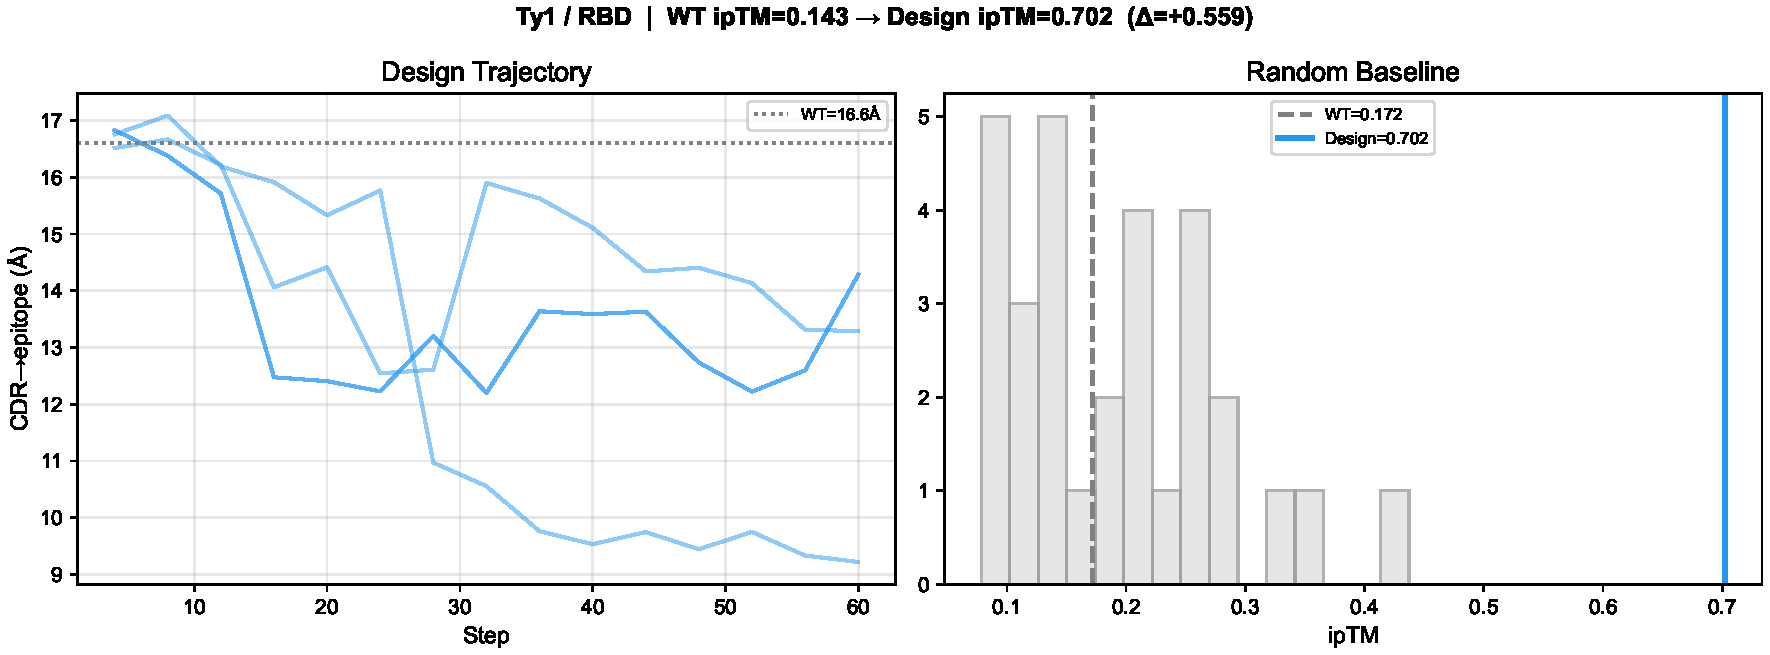
\includegraphics[width=0.48\textwidth]{figures/fig4_RBD_6ZXN_TY1.pdf}\hfill
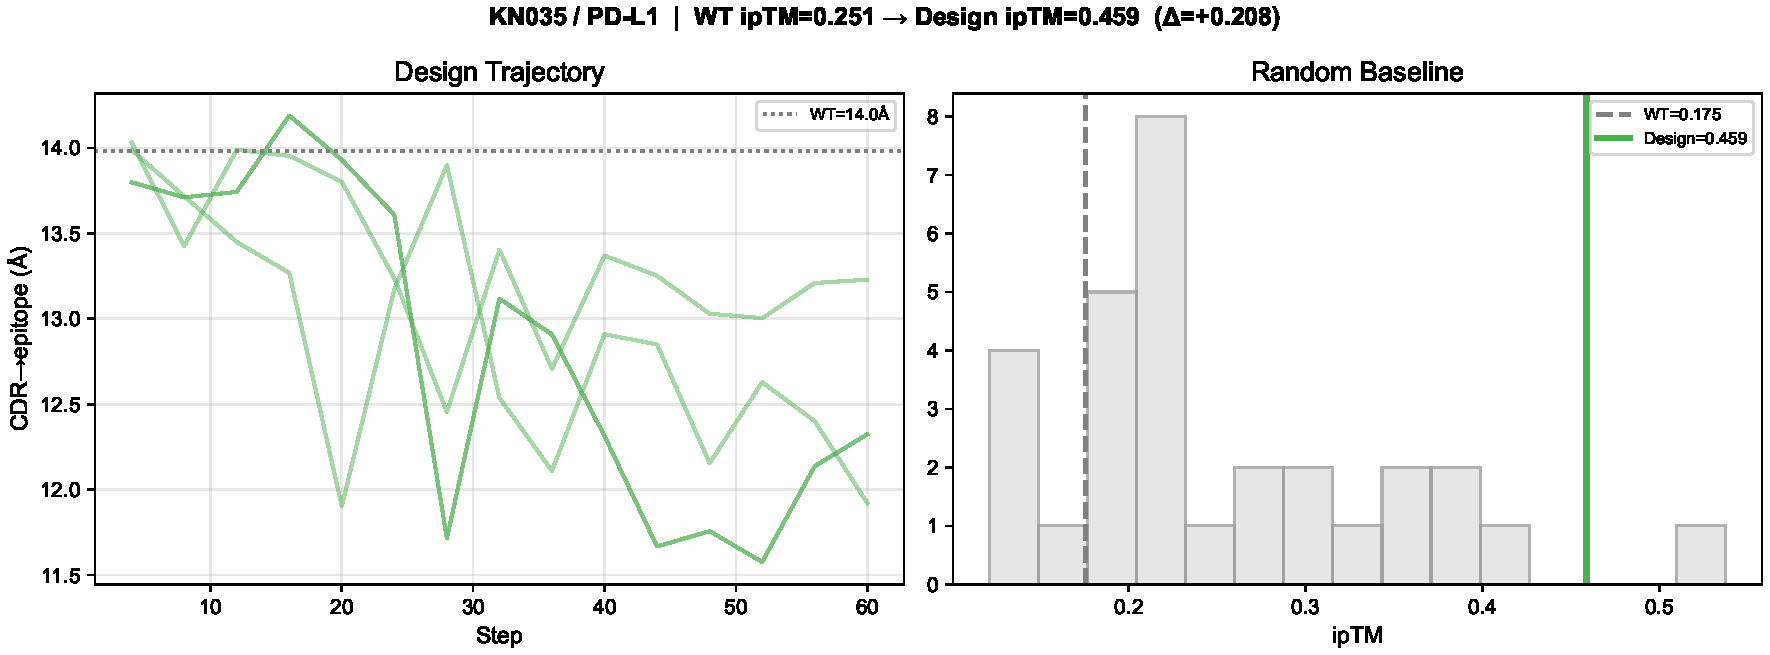
\includegraphics[width=0.48\textwidth]{figures/fig4_PDL1_5JDS.pdf}
\caption{Per-target design trajectory (left) and random baseline distribution (right) for Ty1/RBD and KN035/PD-L1.}
\end{figure}

\subsection{Figure S3: Method overview schematic}

The three-stage pipeline: (1) Full ESMFold2 predicts CA-coordinate structure prior; (2) ESMFold2-Fast serves as differentiable oracle for CDR logit optimization via gradient descent through the distogram; (3) Full ESMFold2 evaluates final candidates.

\section{Supplementary Methods}

\subsection{Extended loss function details}

The complete loss function is:
\begin{equation}
\mathcal{L}_\text{total} = \sum_k w_k \mathcal{L}_k + w_\text{aa} \mathcal{L}_\text{aa\_freq},
\end{equation}
where $k \in \{\text{intra\_contact}, \text{inter\_contact}, \text{glob}, \text{epitope}, \text{structure\_prior}\}$.

\textbf{Intra-contact loss:} Binder internal contact prediction entropy, encouraging well-defined intra-domain contacts.
\textbf{Inter-contact loss:} Binder-target interface contact prediction entropy, encouraging compact interfaces.
\textbf{Global loss:} Global structure quality regularization.
\textbf{Structure prior loss:} Masked cross-entropy between predicted distogram and pre-computed CA prior.

The prior is computed from full ESMFold2 CA coordinates averaged over 4 diffusion samples. CA distances are discretized into 64 bins spanning \SIrange{2}{22}{\angstrom}, with a bin tolerance of \SI{2.5}{\angstrom}.

\subsection{ESMFold2 pose basin analysis}

Our earlier investigation revealed that ESMFold2's predicted complex pose is a deterministic function of the framework sequence, not a sample from a distribution. This was confirmed by: (1) multiple independent folds of the same sequence producing poses within \SI{1.84}{\angstrom} binder RMSD of each other; (2) injecting a \ang{30}-rotated binder pose at the diffusion start having no effect on the final output; (3) comparing framework-variant vs.\ CDR-variant predictions, where framework changes shift the pose by \SI{0.29}{\angstrom} but CDR changes produce \SI{2.54}{\angstrom} variation. This finding underlies our strategy: we keep the framework fixed and optimize only CDRs.

\end{document}
